\documentclass[12pt]{article}

\usepackage[english]{babel}
\usepackage[utf8x]{inputenc}
\usepackage{pdfpages}
\usepackage{lastpage} % Required to determine the last page for the footer
\usepackage{extramarks} % Required for headers and footers
\usepackage{graphicx} % Required to insert images
\usepackage{listings} % Required for insertion of code
\usepackage{courier} % Required for the courier font
\usepackage{color}
\usepackage{grffile}
\usepackage{float}

% Margins
\topmargin=-0.45in
\evensidemargin=0in
\oddsidemargin=0in
\textwidth=6.5in
\textheight=9.0in
\headsep=0.25in
\fboxsep=0mm%padding thickness
\fboxrule=2pt%border thickness

\linespread{1.1} % Line spacing

\newcommand{\Title}{Software requirement specification} % Assignment title
\newcommand{\Class}{Cos\ 301} % Course/class

\begin{document}

	\vspace{4em}
	
	\begin{center}%
	
		\begin{figure}[ht!]
			\centering
			
\includegraphics{./Pictures/logo.png}
	 	\end{figure}
		\LARGE \bf \Title \\
		{\bf Version 0.5}\\[4em]
	  	\LARGE {\bf SoftServe Group }\\[1em]
	  	\LARGE {\bf Members:}\\[2em]
	  	\large
	     Kgothatso Phatedi Alfred Ngako	(12236731) \\[1em]
	     Tokologo “Carlo” Machaba			(12078027) \\[1em]
	     Mathys Ellis						(12019837) \\[8em]
	    
	\end{center}%
	
	\newpage
		{\LARGE \bf Change log}\\[2em]
		
		\begin{tabbing}
			\hspace*{2.5cm}\=\hspace*{2.5cm}\=\hspace*{8cm}\=\hspace*{3cm} \kill
			10/02/2014 \> Version 0.0 \> Document created \> Mathys Ellis \\
			02/03/2014 \> Version 0.1 \> Added to glossary \> Mathys Ellis \\
			04/03/2014 \> Version 0.2 \> Added Integration requirements, Architecture constraints, Functional requirements introduction   \> Alfred Ngako \\
			05/03/2014 \> Version 0.3 \> Added Introduction, Vision, Background, Access Channel requirements \> Carlo Machaba \\
			06/03/2014 \> Version 0.4 \> Added domain objects, open issues. Modified some sections  \> Alfred Ngako \\
			06/03/2014 \> Version 0.5 \> Added quality requirements, methodology, scope and limitations  \> Mathys Ellis \\
			
		\end{tabbing}
	
	\newpage
		\tableofcontents
			
		\listoffigures
	\newpage
	\section{Introduction} %Carlo
	Post-Doctoral fellow a person who conducts research after they have completed their doctoral studies, with the aim of deepening their knowledge in a specific field. The University of Pretoria has a number of post doctoral fellows who conduct their research under the supervision of somebody in the University, and a large portion of this research is funded by the university. 
	\vspace{0.2in}

		\subsection{Purpose:}
		\vspace{0.2in}
		 
	
		\vspace{0.2in}
	
		\subsection{Document Conventions:}
		\vspace{0.1in}
		\begin{itemize}
			\item Documentation formulation: LaTeX
			\item ERD Crow-Foot notation
			\item UML 2.0
		\end{itemize}
	
		\vspace{0.2in}
	
		\subsection{Project Scope:}
		\vspace{0.2in}		
		
		\vspace{0.2in}
	
		\subsection{References:}
		\vspace{0.1in}
			
	
	\vspace{0.5in}
	
	\newpage
	\section{Vision} %Carlo	
	\vspace{0.2in}
	The client simply needs a system which can make the application process of Post Doctoral fellows run smoother. The system will include an easy to use web interface for the applicants and an application for all the stakeholders involved in the rest of the application process. As soon as a step is concluded the system will forward the documentation to the next stakeholder in the process. By introducing a system that is not paper based, the client hopes that the application process will be easier to track on the side of the applicant. The system will also provide better reporting, tracking, audit-ability and accountability with regards to all the other stakeholders involved in the application process. The system needs to be centralised to ensure access to documents and/or information for the different stakeholders
	\vspace{0.5in}
	
	\section{Background} %Carlo
	\vspace{0.2in}
	The current Post-Doctoral application process is paper based and with this a number of problems have been experienced. There is no audit trail when it comes to the different departments involved in approving or declining the applications, minutes of meetings are often misplaced or typed in an inconsistent manner making it hard to recall what has been discussed in the meetings that take place during the application process. Access to documents is a problem since their are a number of different stakeholders, the process of getting hold of the documents is long and often tedious.The reporting of the number of fellows, renewals, communication with fellows and the number of fellows in each department is also a problem, because the current process is not centralised and gathering all the information required to generate reports is a problem.
	\vspace{0.5in}
	
	\newpage
	\section{Methodology} %Mathys
	\vspace{0.2in}
	
	This document was created using the requirement elicitation techniques and requirement definitions specified in Klaus Pohl’s book Requirements engineering (See references).
	The requirements were elicitated from the following sources:
	\begin{itemize}
		\item Numerous interviews with the client
		\item Collecting and analysing various documents such as:
		\begin{itemize}
			\item The initial project request document
			\item Application forms
			\item Renewal forms
			\item CV templates
			\item Approval and recommendation forms			 
		\end{itemize}		
		\item Online research into UP Post doctoral applications
		\item Correspondence with the UP IT department
	\end{itemize}	
	
	\vspace{0.5in}
	
	\newpage
	\section{Architecture requirements}
		\subsection{Access channel requirements} %Carlo
		\vspace{0.2in}
		\begin{itemize}
		\item Post-Doctoral Applicants: Will access the system through a web browser client which will be compatible with the web browsers found in modern phones. 
		\item Other Stakeholders: Will access the system through a Java application found on the computers used by them in their offices.
		\item % Will the UP system interact/access our system?
		\end{itemize}

		\vspace{0.2in}
		
		\subsection{Quality requirements} %Mathys
		\vspace{0.2in}
		
		\subsubsection{Availability:}
				
		\begin{flushleft}
		
		The system's availability on designated networks will depend on the availability of the University of Pretoria's servers that host the system. If the University of Pretoria's servers hosting the system are active and provide access over a designated network then the system must be available over that designated network. The designated networks are defined as the internet and the campus network of the University of Pretoria.
		
		\end{flushleft}
		
		\vspace{0.1in}
				
		\subsubsection{Security requirements}
		
		\begin{flushleft}
		
		The system will need to be fully secured since the system deals with confidential information such as person information, application statuses, financial data and meeting information. Also since the systems main goal is to provide a stable audible application process flow the system may not be vulnerable to data tampering or any tampering whatsoever. \\
		\vspace{0.1in}
		  
		The system will have to provide different security roles to the registered users on the system. In essence a stakeholder may only have access to their section of the application process. The system administrator should be able to view all the sections in the system and should be able to modify them except where they may not.
		
		\end{flushleft}
		
		\vspace{0.1in}
		
		\subsubsection{Scalability requirements}
		
		\begin{flushleft}
		
		The current aim is to create a scalable system that can support 500 to 1000 applicants per year with possible growth. This is in line with the figures given by the client and the growth in the research sector of the university.\\
		\vspace{0.05in}
		
		The system needs to be scalable in regard to the following factors:
		\begin{itemize}
		
		
		\item\textbf{Performance:} This is regarded as the speed and responsiveness of the system.		
		The system needs to be handle report queries in less than 10 seconds. It should be able to handle any application section processing in less than 3 seconds.\\
		
		\item\textbf{Storage:} This is regarded as the growth and shrinking of the data that is stored.
		The system will need to be able to handle a database that is in the range of 1 GB to 15 GB that has the potential to grow even larger.  The reason for this stems from the requirement that the system will support archival functionality and archived data will store the data for long periods of time.\\
		 
		\item\textbf{Concurrency:} This regarded as the amount of active users on the system at the same time.		
		The system will need to support at least 100+/- concurrent users efficient and effectively since the system requires multiple stakeholders to part take in the application process while there can be multiple applications occurring at the same time.\\ 
		 
		\end{itemize}
		\end{flushleft}
		\vspace{0.1in}
		
		\subsubsection{Testability:}
				
		\begin{flushleft}
		
		The system must be testable. This will be done using unit testing and following the test plan that will be laid out in the testing document of this project.\\
		
		\vspace{0.1in}
		
		Unit testing will test each unit in regard to:
		\begin{itemize}
		
		\item\textbf{Preconditions}
		\item\textbf{Post conditions}
		
		\end{itemize}
		
		The project will also have two phases of testing:
		
		\begin{itemize}
		
		\item\textbf{Offline:} This is the initial phase of testing and debugging which will be done with pseudo data.
		\item\textbf{Online:} This is the final phase of testing and debugging which will be done with active real time data.
		
		\end{itemize}
		
		\end{flushleft}
		
		\vspace{0.1in}
		
		\subsubsection{Auditability:}
				
		\begin{flushleft}
		
		The system needs to provide an audit trail of all critical actions that occur in the system. Critical actions are considered: user account management operations, login action, logout action and any operation by a user that leads to a change in application data of a particular prospective fellow.\\
		
		\vspace{0.1in}
		
		The Audit trail will be in the form of a read-only table stored in the database. It can only be viewed by a user with the correct security role. The system is the only entity that can modify the audit trail where this modification can only be the addition of entries.
		
		\end{flushleft}
		\vspace{0.1in}	
		
		\subsubsection{Usability requirements}
		
		\begin{flushleft}
		
		The primary language of the system will be South African English. Any other language support is not considered part of the requirements but the system will be designed to allow for such development in the future.\\
		
		\vspace{0.1in}
				
		The system's UI will only consider 2 types of user categories with regard to usability:
		
		\begin{itemize}
		
		\item\textbf{Trained user:}
		
		This type of user will have to have training in understanding how the system functions and how to use it. Their computer skills will be assumed to be in the range of basic to intermediate. Thus the user interface can allow for certain complexities but these complexities must be kept at a minimal. This user will be regarded as a system administrator.  The stakeholders who fall under this category is the DRIS staff members overseeing the application process.
		
		\item\textbf{Normal user:}
		
		This type of user will have no training. Their computer skills will be assumed to be none or minimal. Therefore the UI that they will have access to will be simplistic and will be as user friendly as possible. The stakeholders that fall under this category will be Prospective fellows, Grant holders, HODs, Deans and Post-doctoral committee members.
		
		\end{itemize}
		
		\end{flushleft}
		
		\vspace{0.2in}	
		
		
		\subsection{Integration requirements} %Alfred
		\vspace{0.2in}
		The system has to integrate with the following systems:
		\begin{itemize}
			\item A MySQL database.
			\item A mobile (android) application used to record minutes of the meetings by the stakeholders. 
			\item An emailing service? %I need to recitfy this a bit.
			\item Adobe API used when generating reports.
			\item Must be able to access and utilize the NRF researcher ratings.
		\end{itemize}
		\vspace{0.2in}
		
		\subsection{Architecture constraints} %Alfred
		\vspace{0.2in}
		The following architecture constraints have been selected as being suitable for the system.
		\begin{enumerate}
			\item Database technology: MySQL
			\item Development technology: Java EE
			\item Web server: Apache Tomcat.
			\item Application server: GlassFish 
			\item It must run using HTTPS requests and response events to connect to the
database.
		\end{enumerate}
		\vspace{0.5in}
	
	\newpage	
	\section{Functional requirements}
		\subsection{Introduction} %Alfred
		\vspace{0.2in}
		This section discusses the functional requirements for the University of Pretoria's Post Graduate application system. Highlighting the scope and limitations that are faced by the system. \linebreak \linebreak
		The required functionality, domain objects and use cases related to the functional requirement will be discussed. 
		\vspace{0.2in}
		
		\subsection{Scope and Limitations/Exclusions} %Mathys
		\vspace{0.2in}
			
		
		\subsubsection{Scope}
		\vspace{0.2in}
		
			\begin{figure}[H]
				\centering				
				\framebox{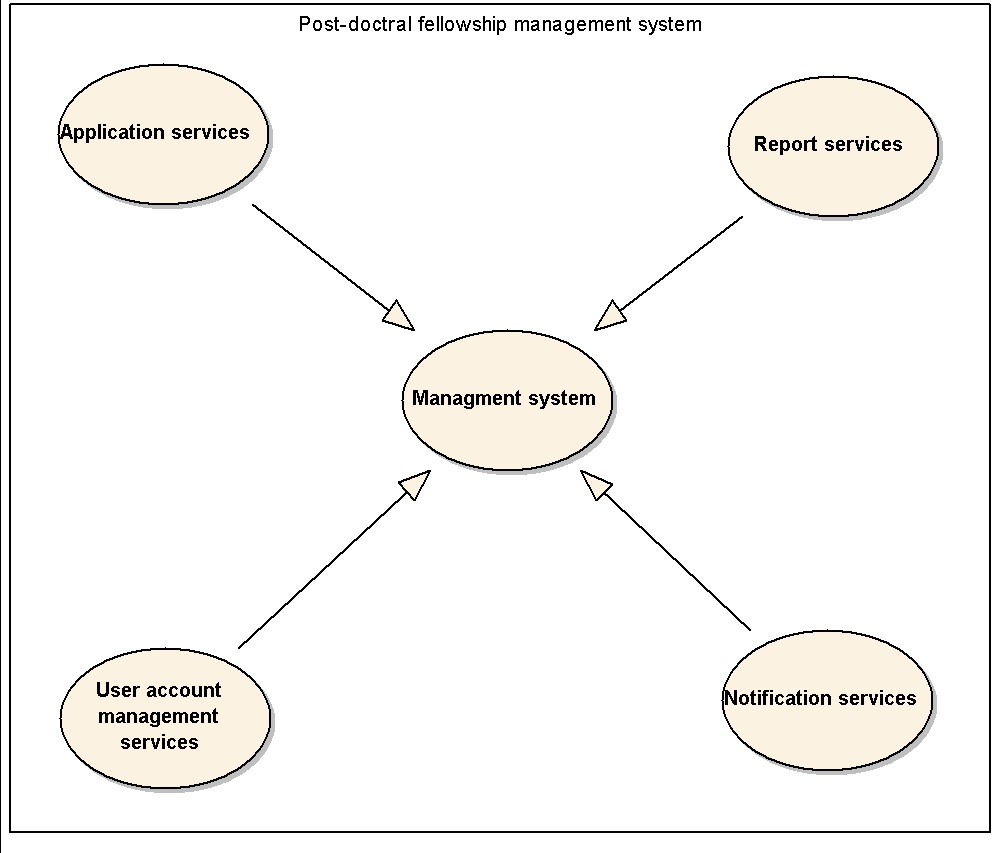
\includegraphics[scale=0.6]{./Pictures/Diagrams/Post-doctral fellowship management system.jpg}}
				\caption{Use case diagram of Post-doctoral fellowship management system}
			\end{figure}
			
			\begin{figure}[H]
				\centering				
				\framebox{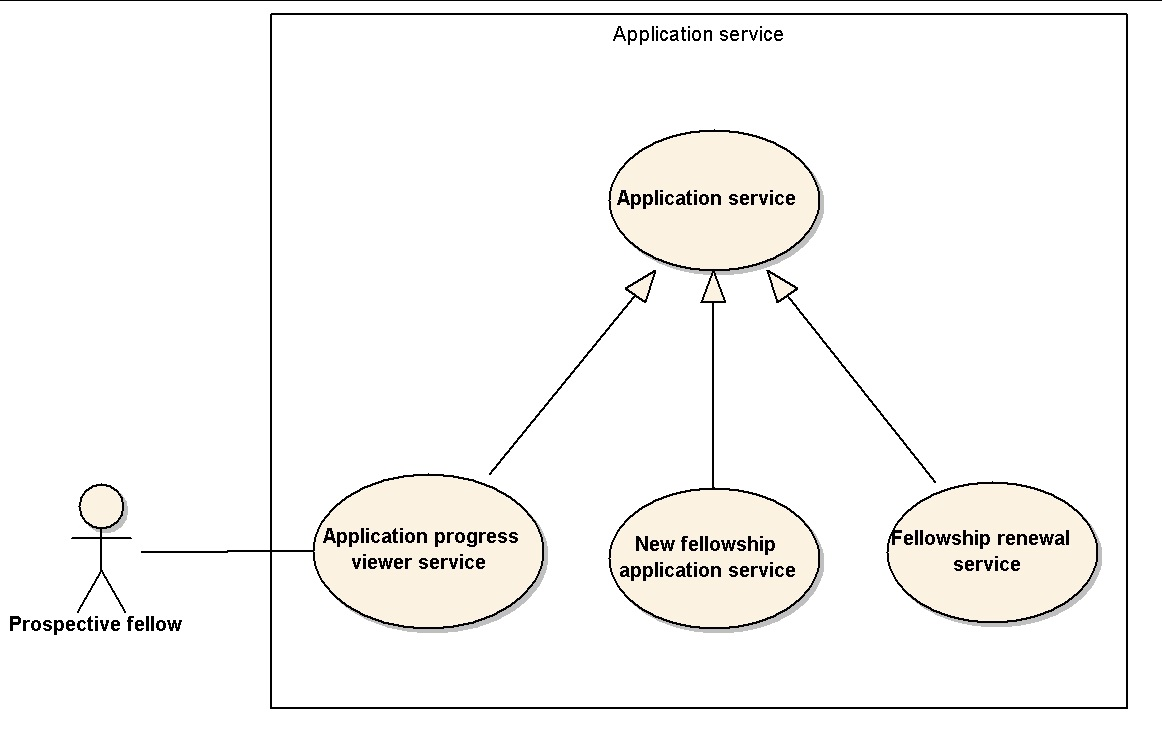
\includegraphics[scale=0.6]{./Pictures/Diagrams/Application service.jpg}}
				\caption{Use case diagram of Application service}
			\end{figure}
									
			\begin{figure}[H]
				\centering				
				\framebox{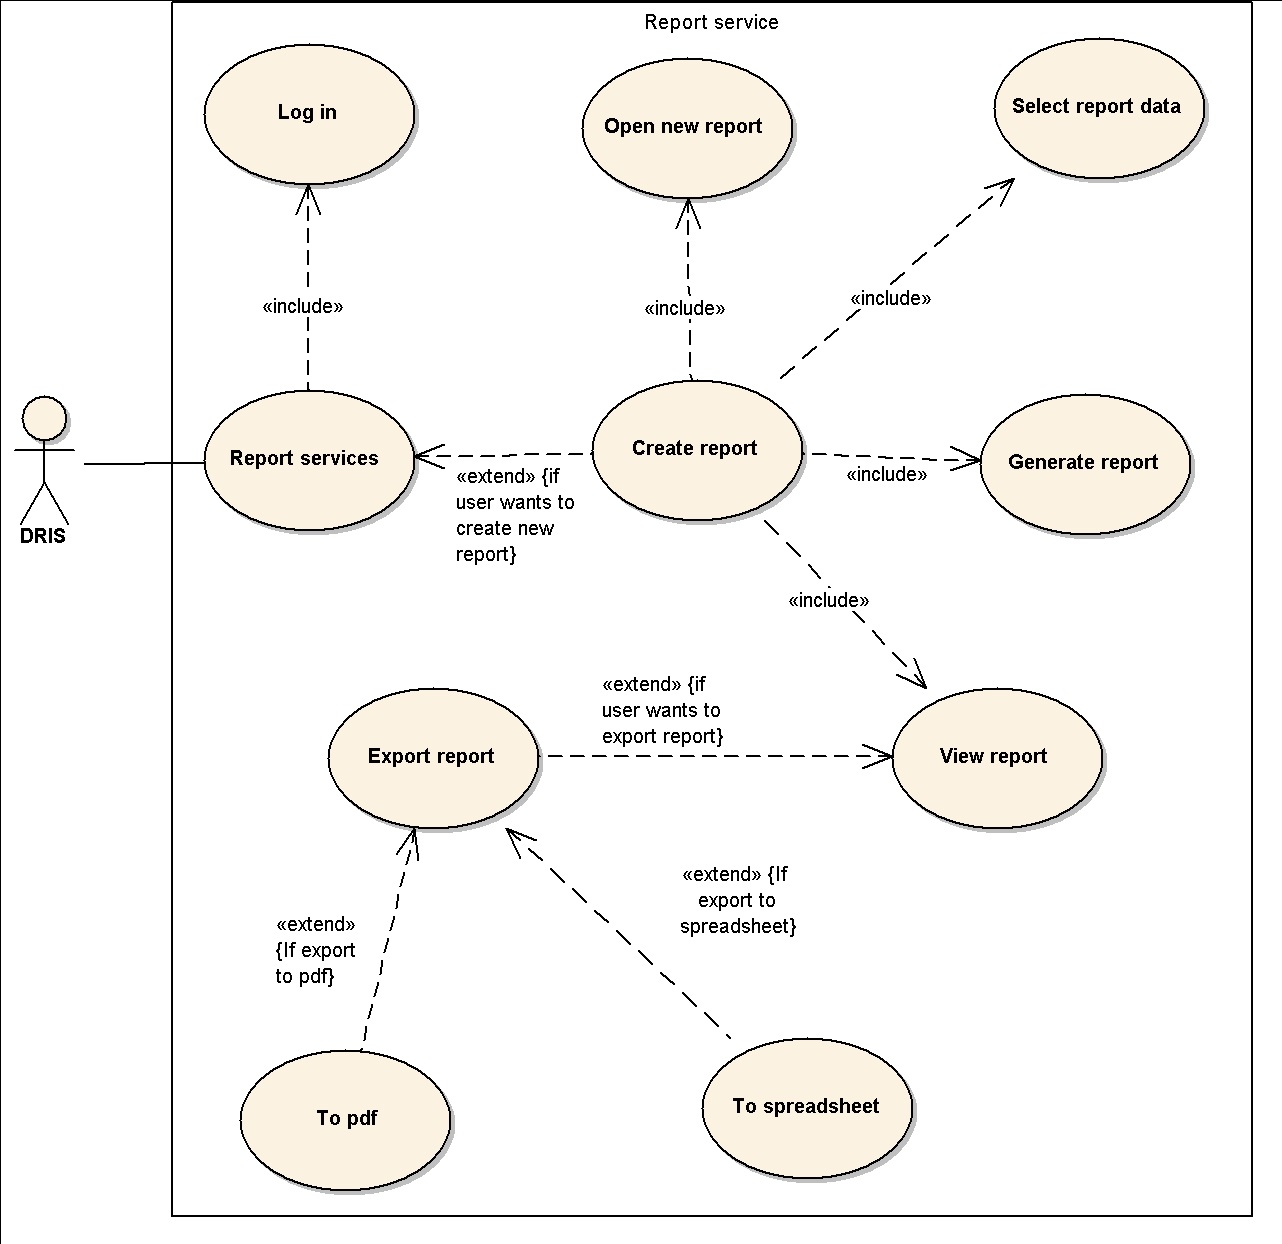
\includegraphics[scale=0.6]{./Pictures/Diagrams/Report service.jpg}}
				\caption{Use case diagram of Report service}
			\end{figure}
			
			\begin{figure}[H]
				\centering				
				\framebox{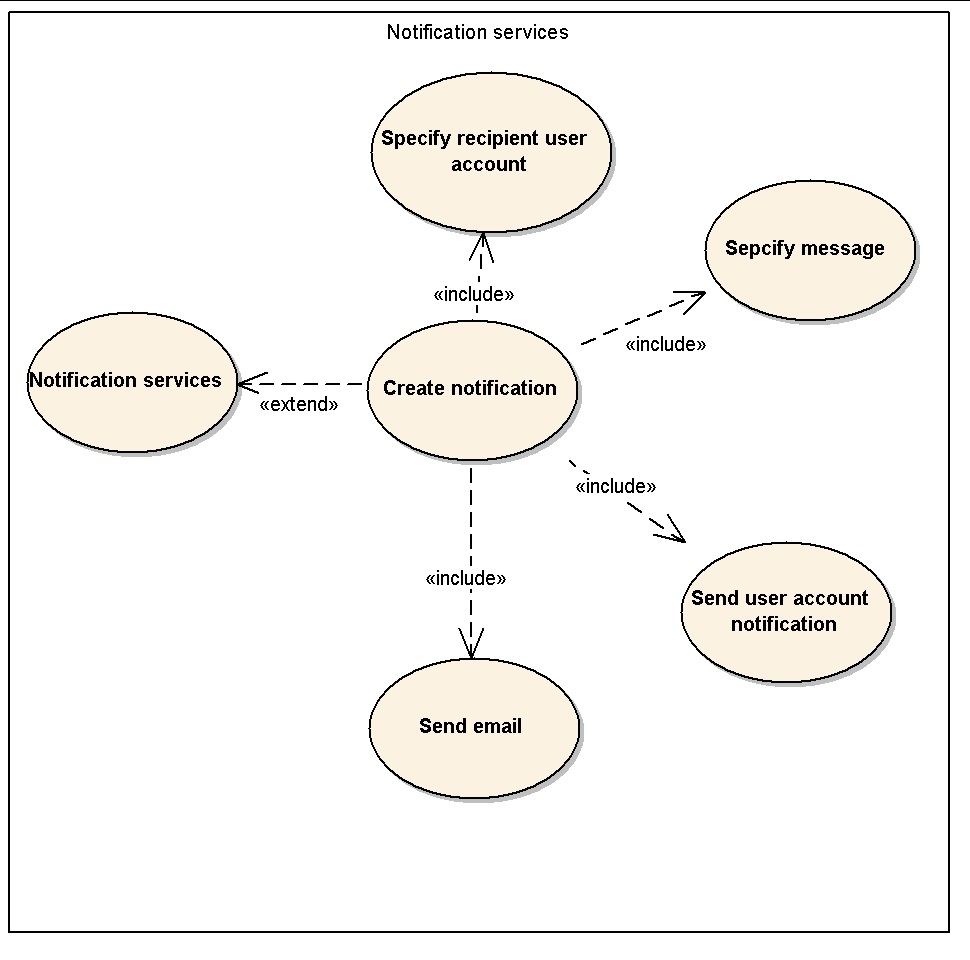
\includegraphics[scale=0.6]{./Pictures/Diagrams/Notification services.jpg}}
				\caption{Use case diagram of Notification services}
			\end{figure}
			
			\begin{figure}[H]
				\centering				
				\framebox{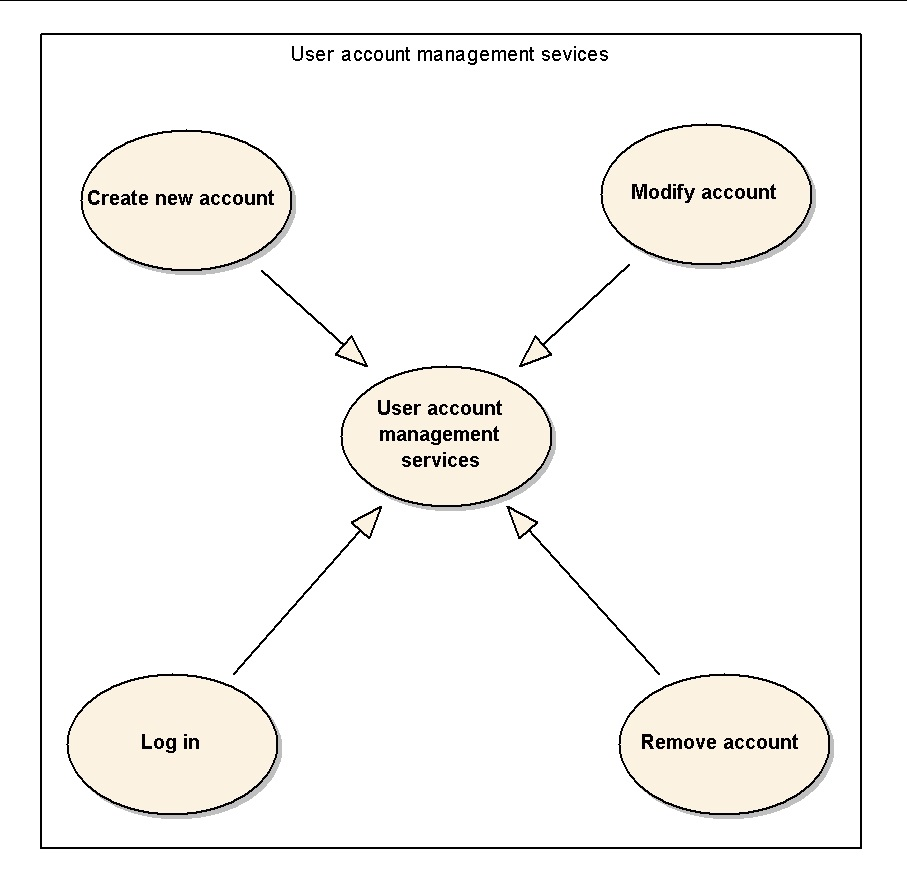
\includegraphics[scale=0.6]{./Pictures/Diagrams/User account management services.jpg}}
				\caption{Use case diagram of User account management services}
			\end{figure}
			
			\begin{figure}[H]
				\centering				
				\framebox{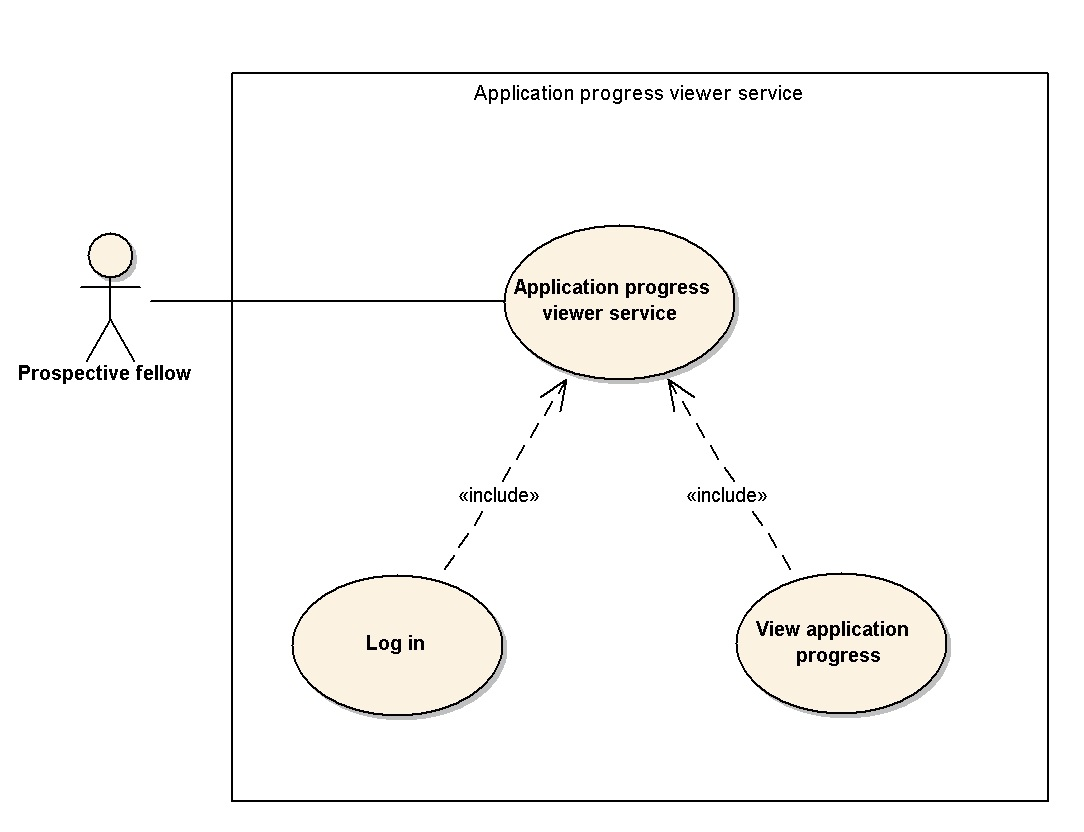
\includegraphics[scale=0.6]{./Pictures/Diagrams/Application/Application progress viewer service.jpg}}
				\caption{Use case diagram of Application progress viewer service}
			\end{figure}
			
			\begin{figure}[H]
				\centering				
				\framebox{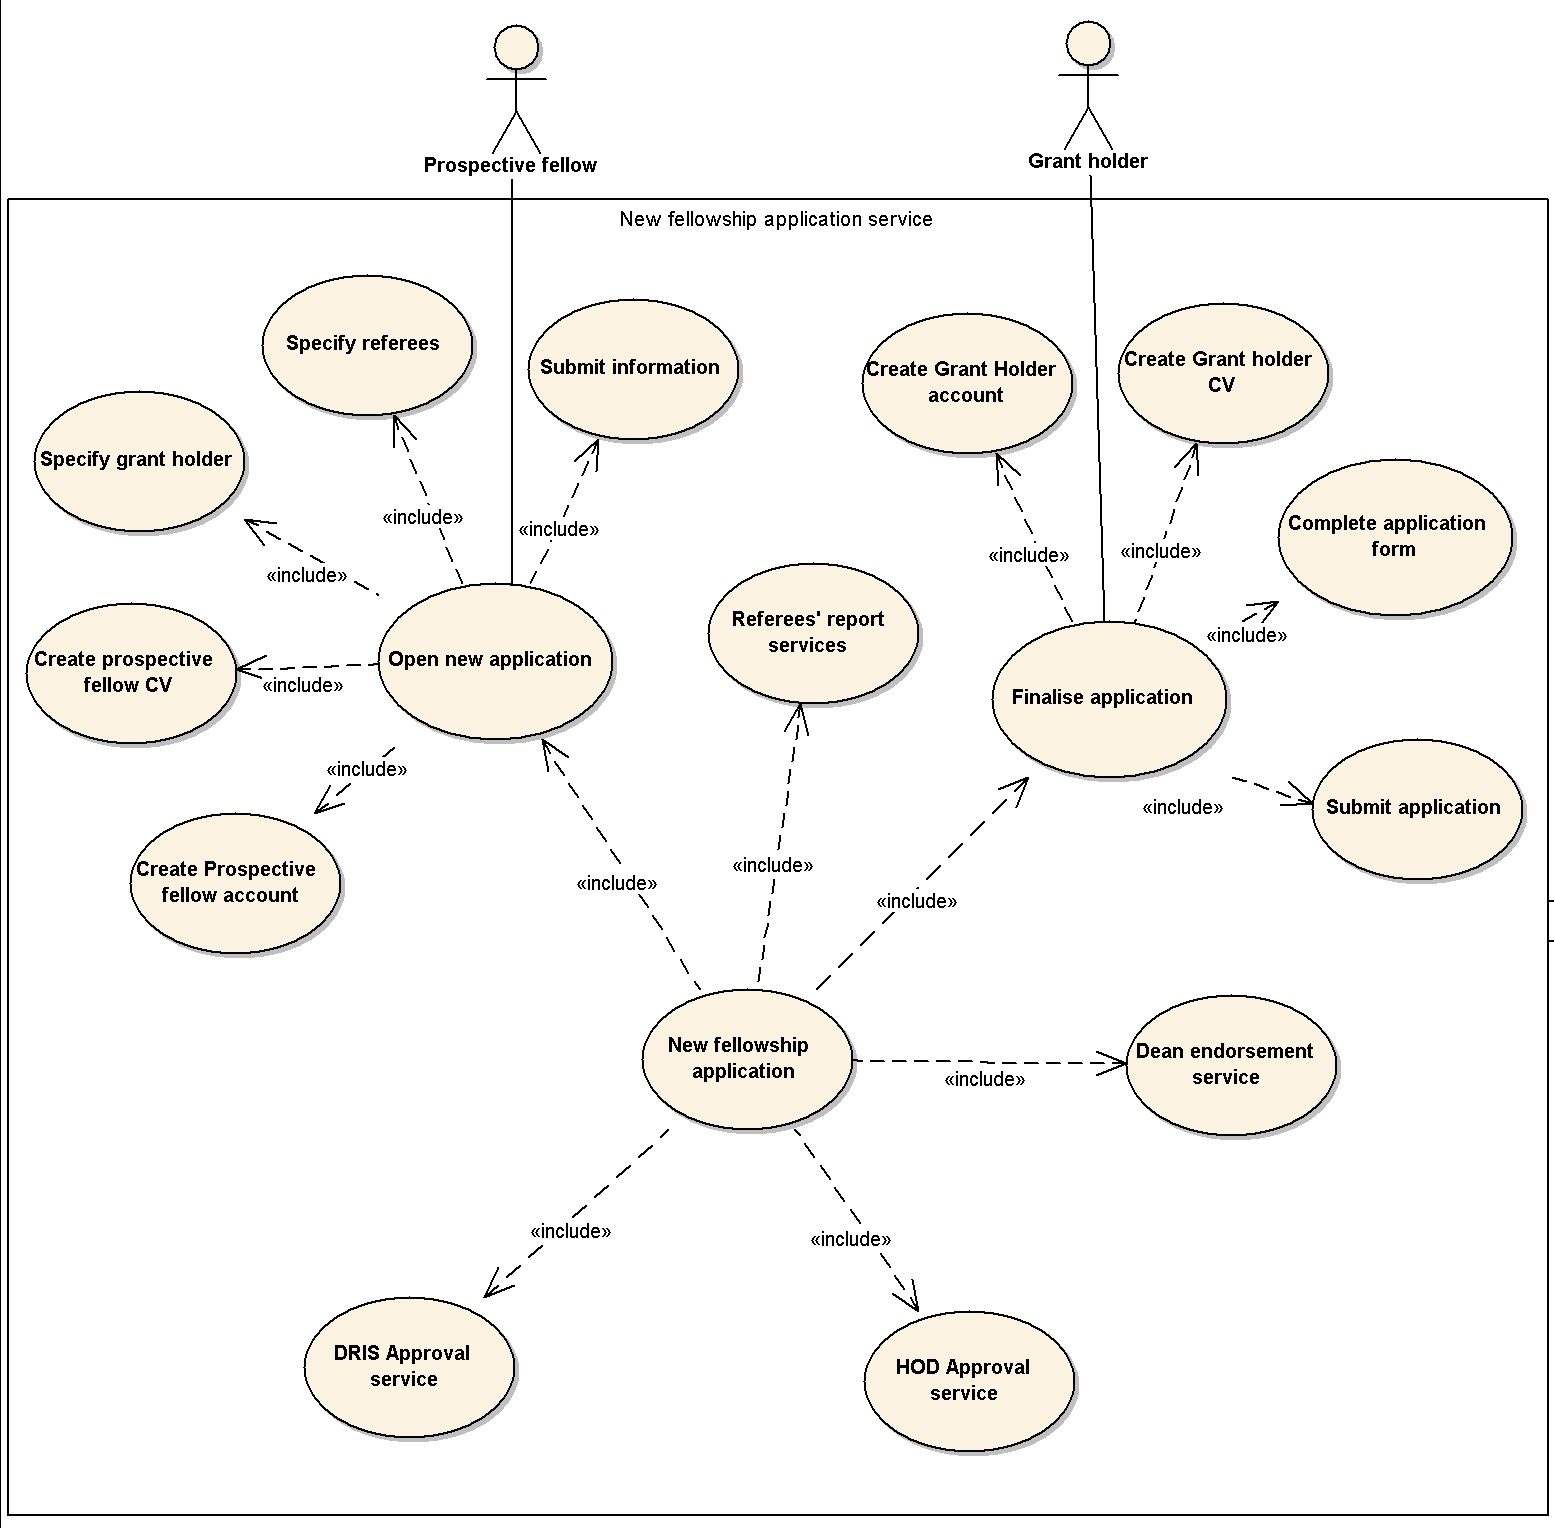
\includegraphics[scale=0.6]{./Pictures/Diagrams/Application/New fellowship application service.jpg}}
				\caption{Use case diagram of New fellowship application service}
			\end{figure}
			
			\begin{figure}[H]
				\centering				
				\framebox{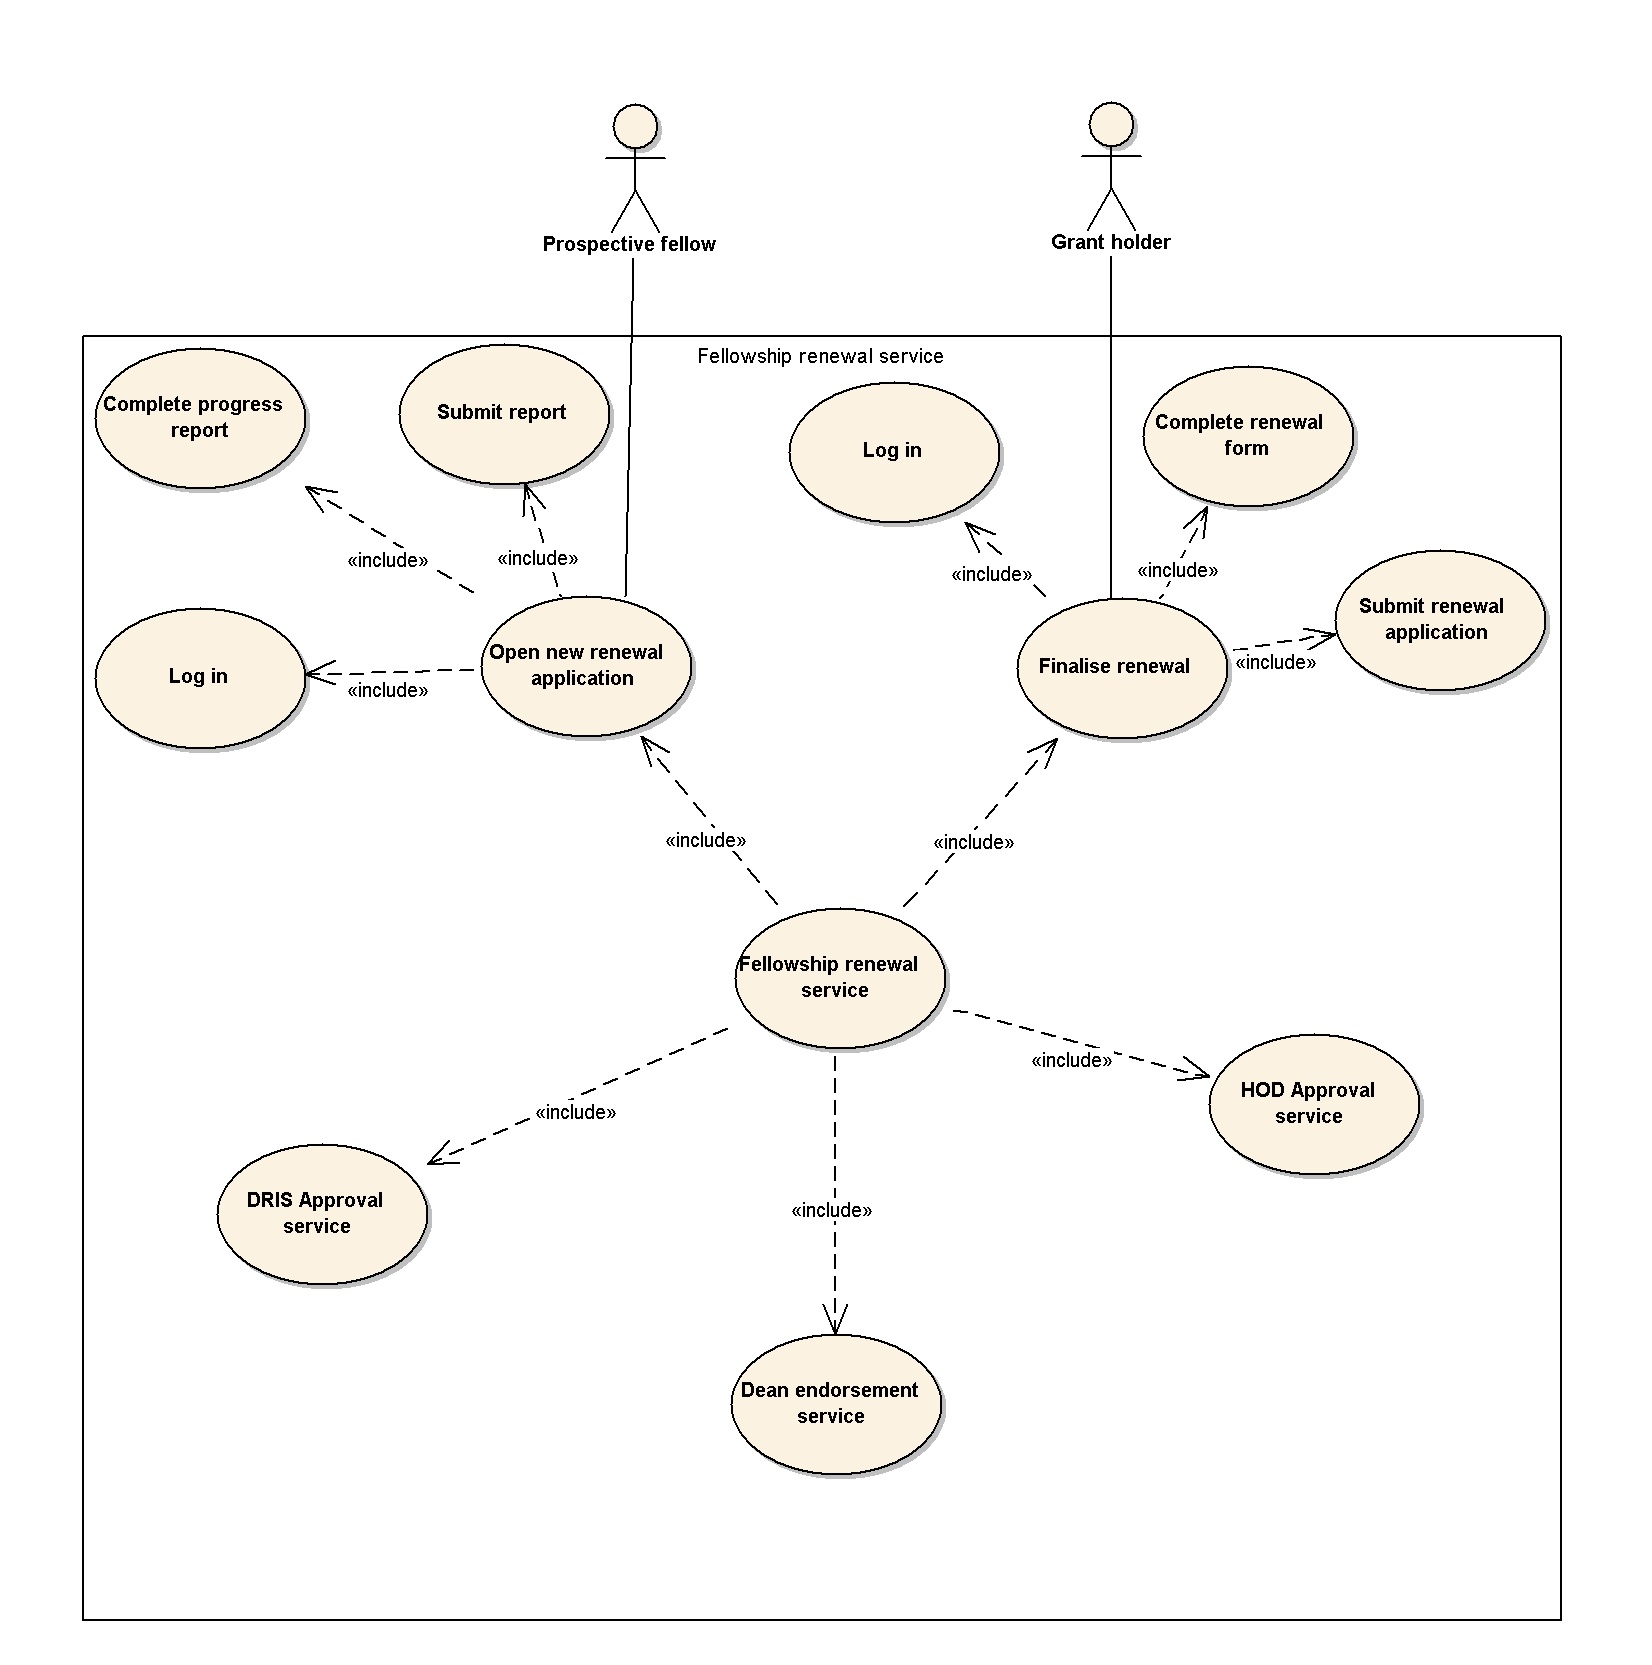
\includegraphics[scale=0.6]{./Pictures/Diagrams/Application/Fellowship renewal service.jpg}}
				\caption{Use case diagram of Fellowship renewal service}
			\end{figure}
			
			\begin{figure}[H]
				\centering				
				\framebox{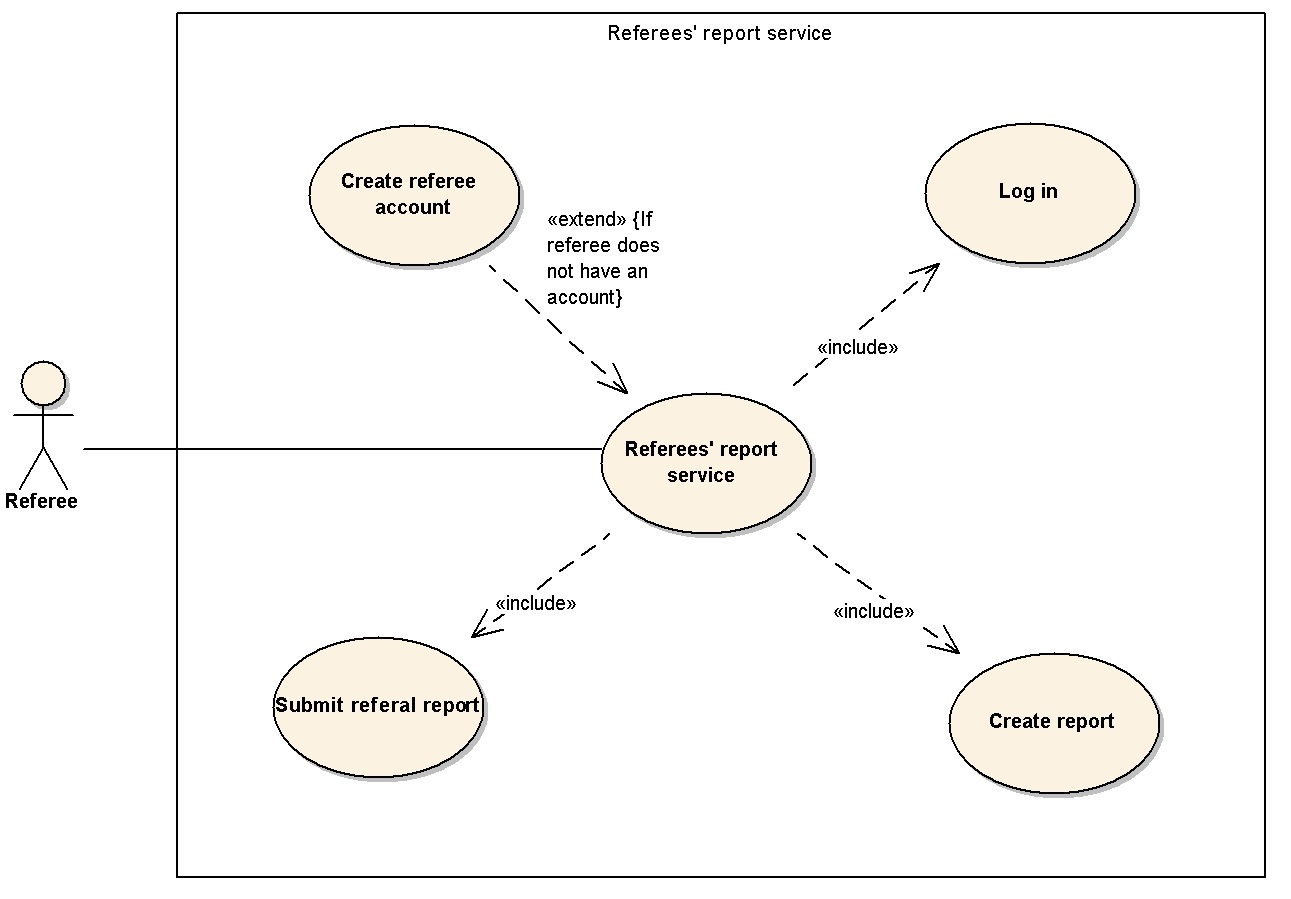
\includegraphics[scale=0.6]{./Pictures/Diagrams/Application/Referees' report service.jpg}}
				\caption{Use case diagram of Referees' report service}
			\end{figure}
			
			\begin{figure}[H]
				\centering				
				\framebox{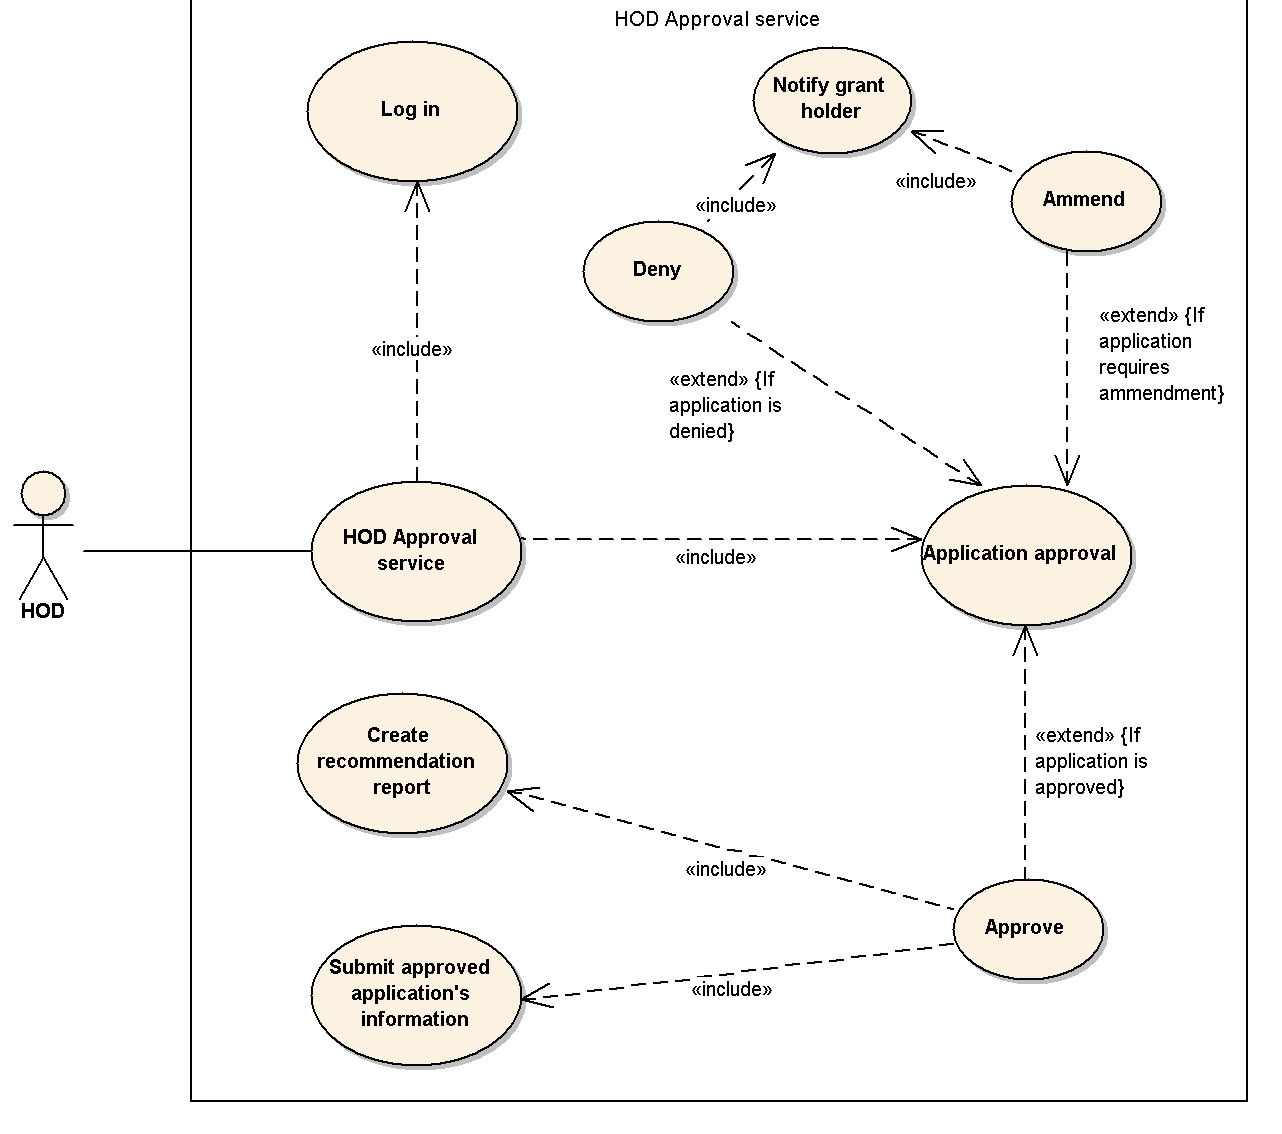
\includegraphics[scale=0.6]{./Pictures/Diagrams/Application/HOD Approval service.jpg}}
				\caption{Use case diagram of HOD Approval service}
			\end{figure}
			
			\begin{figure}[H]
				\centering				
				\framebox{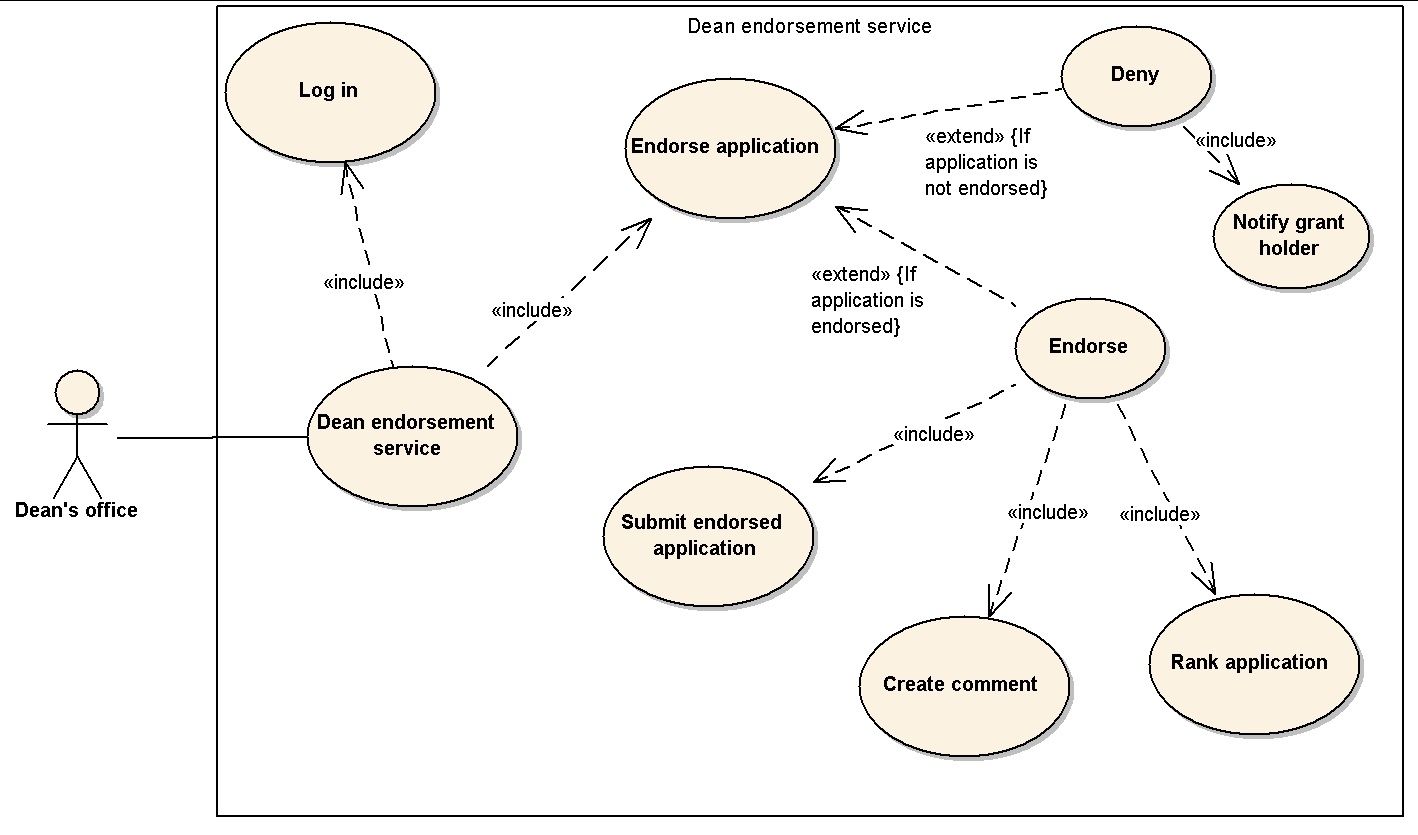
\includegraphics[scale=0.6]{./Pictures/Diagrams/Application/Dean endorsement service.jpg}}
				\caption{Use case diagram of Dean endorsement service}
			\end{figure}
			
			\begin{figure}[H]
				\centering				
				\framebox{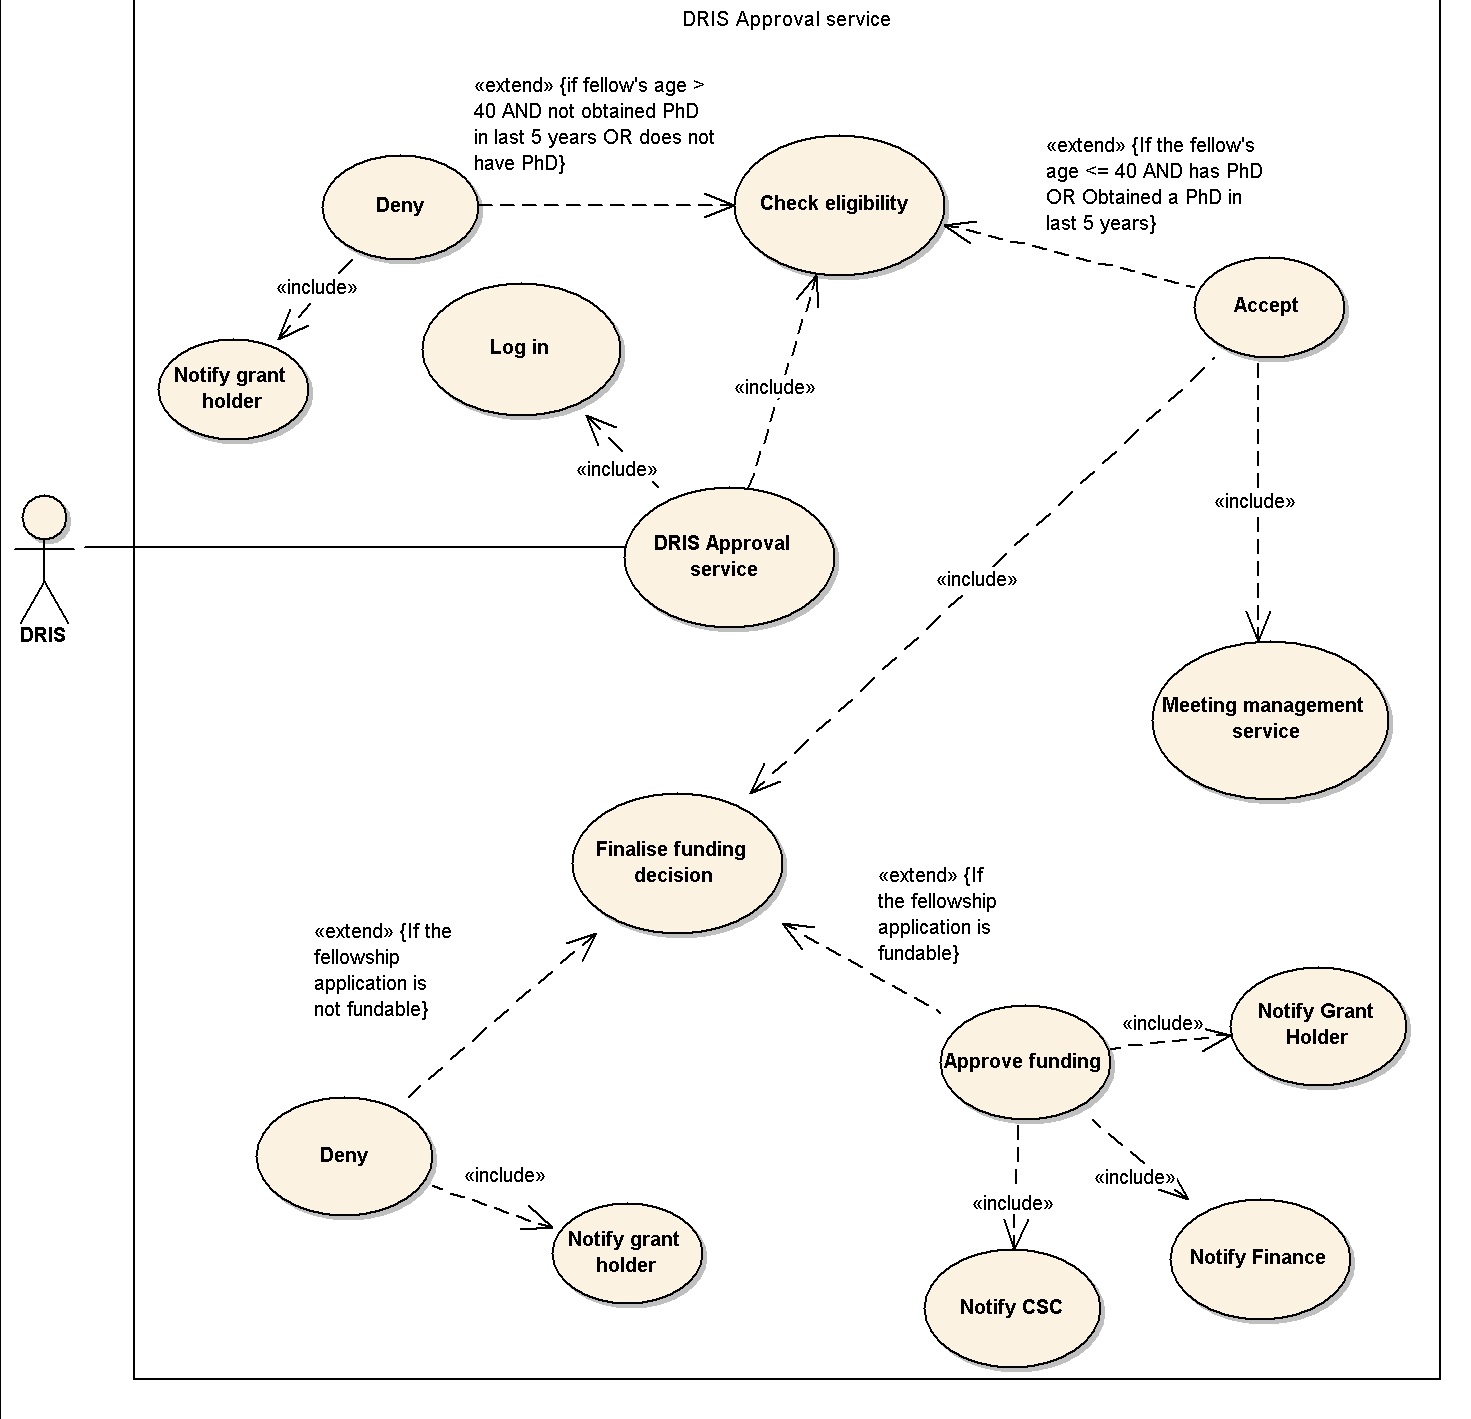
\includegraphics[scale=0.6]{./Pictures/Diagrams/Application/DRIS approval service.jpg}}
				\caption{Use case diagram of DRIS approval service}
			\end{figure}
			
			\begin{figure}[H]
				\centering				
				\framebox{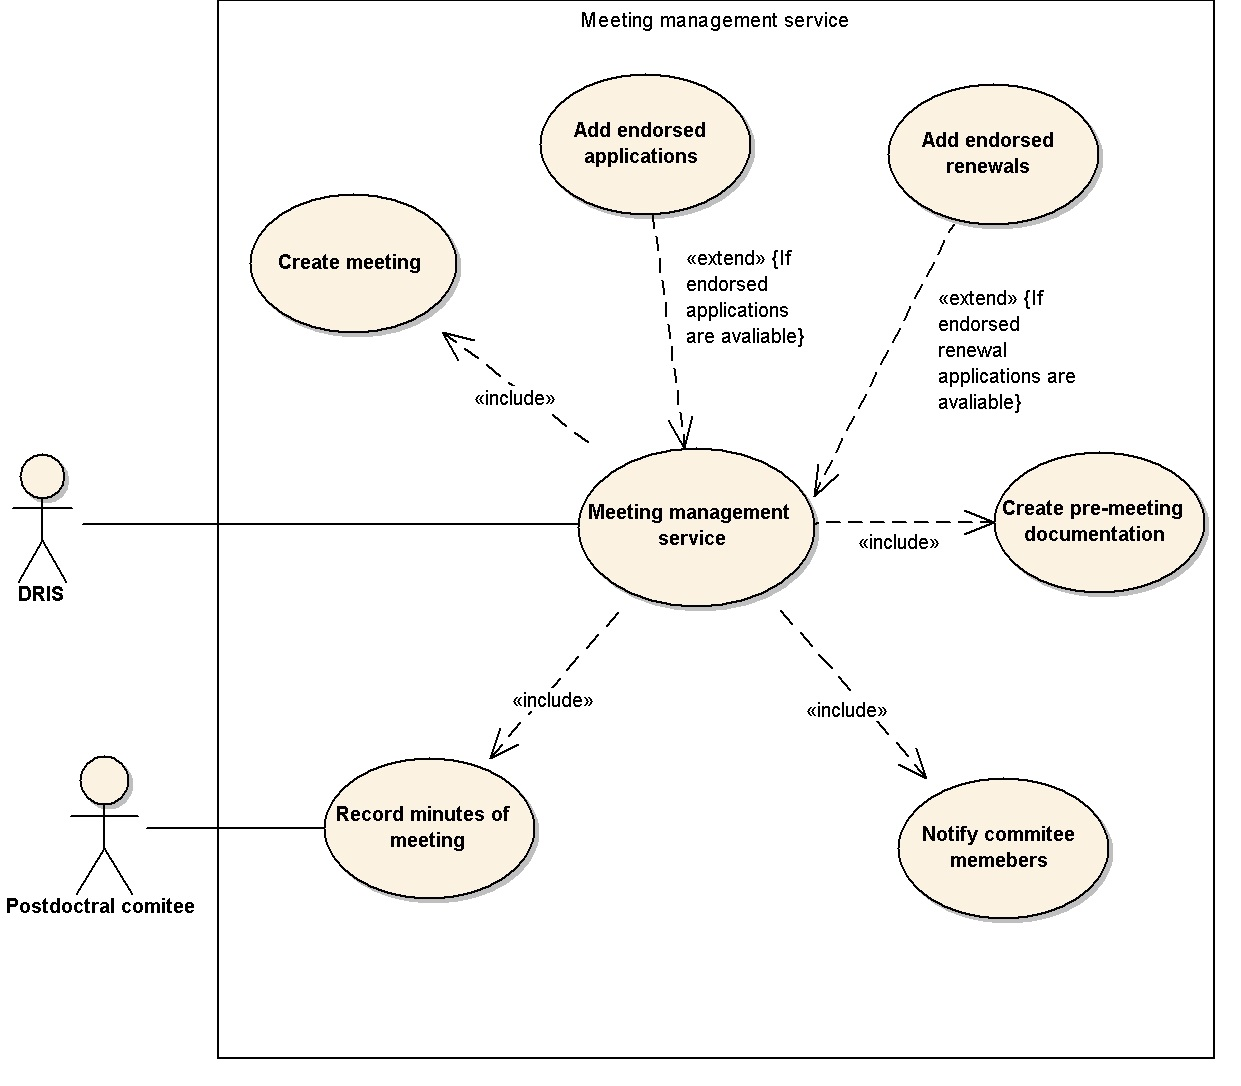
\includegraphics[scale=0.6]{./Pictures/Diagrams/Application/Meeting management service.jpg}}
				\caption{Use case diagram of Meeting management service}
			\end{figure}
		
		\vspace{0.2in}
		\subsubsection{Exclusions}
		\vspace{0.2in}
		
		\vspace{0.2in}
		
		\subsection{Required functionality} %Alfred
		\vspace{0.2in}
		The following sections will discuss the required functionality of all the major processors handled by the system. Namely:
		\begin{itemize}
			\item Application process,
			\item Selection process,
			\item Notification process and
			\item Report process.
		\end{itemize}
		\subsubsection{Application process}
		An application to be research fellow will go through these steps:
		\begin{enumerate}
			\item A potential research helper will need to have/create an account on the system which they will use through their whole application process. 
			\item The account will have a unique username and secured by a user specified password.
			\item Once an applicant is logged on they will then proceed to upload their CV's, academic record and profile. All the information the applicant will provided shall be related to the applicants account. 
			\item The applicant will have to give the names and contact details of at least 2 of his referees, which will than be sent a link via email to fill out a referral form. 
			\item The applicant has to provided information about the supervisor they will be working under throughout their stay as research fellow. The supervisor will be notified via email and either accept or decline the applicant. If the applicant is declined the can try to provide a supervisor again for a maximum of 3 attempts till either accepted or declined by the system.
		\end{enumerate}
		Once the steps are completed the applicants application is now under consideration. The applicant will also be able to see the status of the the applications current state through the whole consideration phase.
		\subsubsection{Selection process}
		The application will now go through a chain of various stakeholders, namely... , who will either approve or decline the application. If the application is declined, reason to why it was declined can be provided to allow the applicant to rectify the issue and continue with the application. If an application is approved, it will then be forward on to the next stakeholder in the system.
		\subsubsection{Notification process}
		Every participant is due to receive notifications regarding their actions every now and then.
		\subsection{Report process}
		The report use cases provides the uses for report generation such as the generation of an applications current status, the 
		\subsubsection{Meeting minutes} % Can't seem to think of a better name to describe the council meetings.
		The post-doctoral committee will on occasion hold meetings and the minutes of those meetings will be centerilizd in this system.
		\vspace{0.2in}
		
		\subsection{Use case prioritization} %Alfred
		\vspace{0.2in}
		
		\vspace{0.2in}
		
		\subsection{Use case/Services contracts} %Mathys
		\vspace{0.2in}
		
		\vspace{0.2in}
		
		\subsection{Process specifications} %Alfred
		\vspace{0.2in}
		
		\vspace{0.2in}
		
		\subsection{Domain Objects} %Alfred
		\subsubsection{Overview}
		\begin{description}
			\item[Stakeholder] the full participants who administer the application process. Namely: 
				\begin{itemize}
					\item DRIS
					\item Dean's office
					\item Grant holder
					\item HOD
					\item Post-doctoral committee
					\item Prospective fellow
					\item Referee
				\end{itemize}
			\item[Application] which will be created by prospective fellow. Viewed and supplemented by other stakeholders who will either approve or deny the application.
			\item[Post-doctoral committee meetings] held to discuss issues relating to the postdoctoral system such as ranking and evaluating applicants.
		\end{description}
		\vspace{0.5in}
		\subsubsection{Stakeholder}
		All stakeholders, except referees, will have accounts which they use to log on to the system with a unique username and a predefined or user specified password.\linebreak \linebreak
		Grant holder are possibly rated researchers by the NRF and the system should not require the CV's of A and B rated researchers to be added to the system. The reason for this is that the CV's of such researchers are very long.
		\subsubsection{Application}
		Applications will contain the required info of a prospective fellow, e.g. CV and academic record, and who their researcher leader (grant holder) is. The status of the application will be accessible in reports for all stakeholders. The status will either be under consideration, denied or accepted.
		\subsubsection{Post-doctoral committee meetings}
		The post-doctoral committee will be assessing the applications and will evaluate and give an application a ranking.
		
	\newpage	
	\section{Open Issues:} %Everyone
	\vspace{0.2in}
	
	\begin{itemize}
		\item Theft or loss of mobile devices
		\item User errors like typing errors
		\item How will an applicant be allocated a student number?
		\item Should the system treat a prospective fellow in a unique class or a should all stakeholders be of the same class and be allocated different roles, as someone could work as a stakeholder but still want to apply?
		\item Automating a check for the rating of researchers.
		\item The CVs of A and B rated researchers was not added to save paper. Should we still not add it to keep it more convineint for the researchers?
	\end{itemize}
	
	
	\vspace{0.5in}
	
	\newpage
	\section{Glossary:} %Mathys
	\vspace{0.2in}
	
	\begin{itemize}
		\item \textbf{Prospective fellow} - A person who wishes to apply for a research position
		\item \textbf{Grant holder} - The person who is a fellow's supervisor and a member of staff at the University of Pretoria
		\item \textbf{HOD} - The head of the department under which a Grant holder falls
		\item \textbf{Dean's office} - The dean and deputy dean of the faculty under which the department of the Grant Holder falls
		\item \textbf{DRIS} - The department of Research and Innovation Support at the University of Pretoria
		\item \textbf{Post-doctoral committee} - The committee who evaluates the post-doctoral fellowship applications and renewals
		\item \textbf{CSC} - Client service centre of the University of Pretoria
		\item \textbf{Finance} - The department of finance at the University of Pretoria
		
		\item \textbf{CV} - Curriculum Vita
		\item \textbf{PDF} - Portable Document Format file
		\item \textbf{NRF} - National Research Foundation. 
	\end{itemize}	
		
	
	\vspace{0.5in}
		

\end{document}
